\section{System Architecture Design}\label{sec:system-architecture-design}

In the following we will specify our main components that execute our main functionalities.
All components are separated into the following layers according to ISO/OSI model.

\begin{figure}
    \centering
    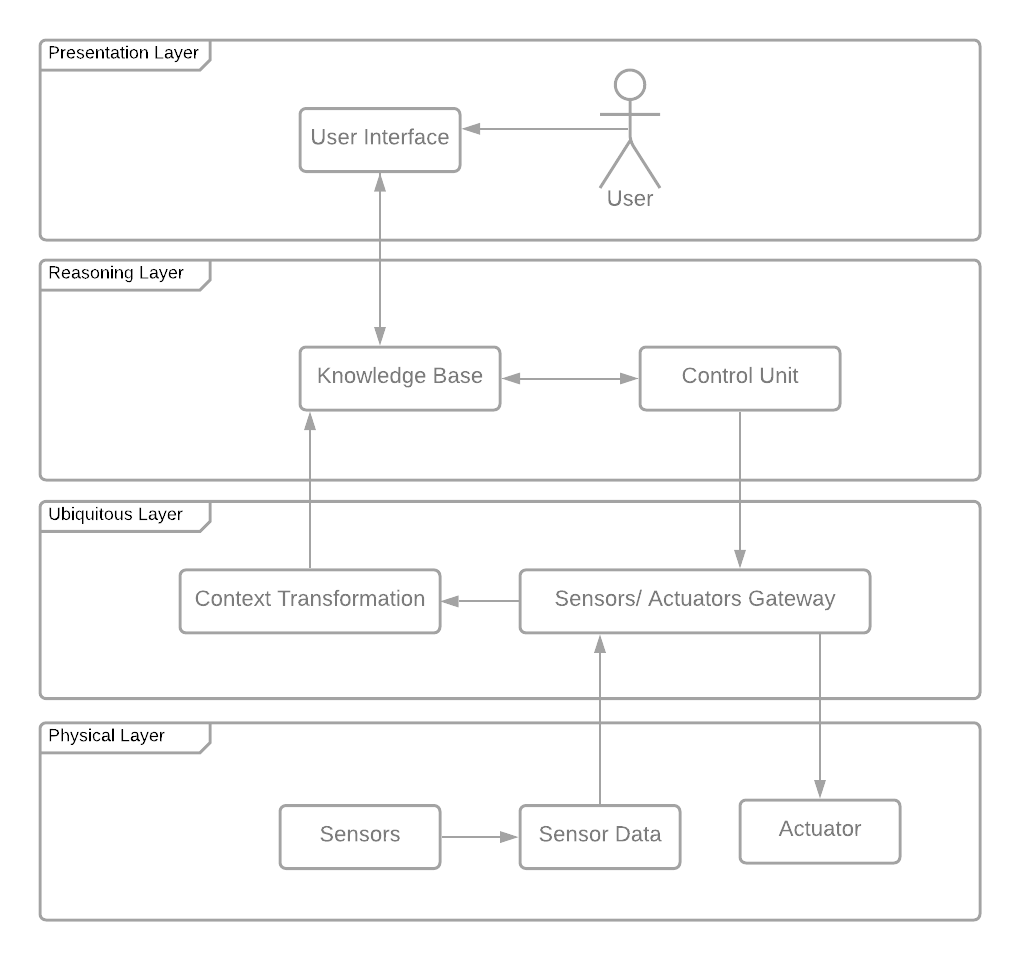
\includegraphics[width=\linewidth]{img/system-design.png}
    \caption{The system design illustrated as a diagram}
    \label{fig:system-design}
\end{figure}

\subsection{Presentation layer}\label{subsec:presentation-layer}
The presentation layer consists of the user interface and the user itself.
The (human) user interacts with our system via the user interface which is a GUI. The user can monitor the system as described in functional requirement FA-5.

\subsection{Reasoning layer}\label{subsec:reasoning-layer}

The reasoning layer consists of the knowledge base, and the control unit.
The knowledge base stores all the sensor data that is generated and stores information about the individual room with the state of all the actuators.
It receives all its data from the context transformation component in the ubiquitous layer.
The control unit interacts closely with the knowledge base, as it loads the measured sensor data from the knowledge base.
Based on this data, the control unit decides based on AI-planning what actions it should take next.
As soon as it has reached a conclusion and formulated a plan, it communicates this plan with the gateway in the ubiquitous layer.

\subsection{Ubiquitous layer}\label{subsec:ubiquitous-layer}

The main component of the ubiquitous layer is the gateway which communicates between the physical layer devices and the components of the reasoning layer.
It will process commands from the control unit of the reasoning layer directly in order to relay commands to the actuators of the system.
Sensor data however will be sent to the context transformation component which will transform the raw data into a more precise and informative format the result is then communicated with the knowledge base of the reasoning layer.

\subsection{Physcial layer}\label{subsec:physcial-layer}

There are two main components of the physical layer.
Firstly the sensor which produces sensor data that will be sent to the gateway.
Sensors will be used to satisfy functional requirements such as FA-8 and others.
Secondly actuators will get instructions from the gateway and execute them as described in the functional requirements.
